\subsection{Project process}

Virtually every projects is bound by time and resource constraints. For us, it is important to showcase the idea and possible uses. To better prioritise, where we put effort and what activities we carry out first, we adopted the \textit{software prototyping} approach. \textit{``A prototype is an initial version of a software system that is used to demonstrate concepts, try design options and find out more about the problem''}~\cite{Sommerville2011SoftwareEngineering}. We use the prototype to demonstrate the novel idea. Prototype development process consists of four steps:
\begin{enumerate*}[label=(\roman*)]
    \item establish prototype objectives,
    \item define prototype functionality,
    \item develop the prototype and
    \item evaluate the prototype~\cite{Sommerville2011SoftwareEngineering}.
\end{enumerate*}

Our project process closely follows the prototype development process, but differs by adding the first step -- \textit{Design the system architecture}. This refined process is shown in Figure \ref{fig:prototype-process}. In the first step of the process, we design the overall architecture of the system so it can serve as a basis for further implementation decisions.

\begin{figure}
    \centering
    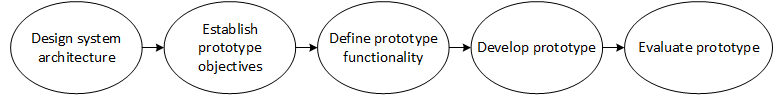
\includegraphics[width=\textwidth]{prototype-process-m}
    \caption{The development process used in this project. Taken from~\cite[p. 45]{Sommerville2011SoftwareEngineering}, edited.}
    \label{fig:prototype-process}
\end{figure}

In the second step, we establish, what do we expect from the prototype. In this project, the aim of the prototype is to demonstrate the idea, therefore as part of establishing the prototype objectives, we define what our idea is with the help of prototype requirement specification (section \ref{sec:system-reqs}, p. \pageref{sec:system-reqs}). 

In the next step, we define the functionality of the prototype, again with the use of requirement specification. However, this step focuses on requirements of individual components separately (section \ref{sec:component-reqs}, p. \pageref{sec:component-reqs}).

In the last step, we evaluate the prototype. We use requirement analysis and test scenario for the evaluation, as described in section \ref{sec:evaluation} (p. \pageref{sec:evaluation}).

This project process resembles the waterfall project model -- indeed we do not return to a previous step during any part of the process, as would be the case with the iterative approach. On the other hand, shall the product ever be released to the market, more work would be needed in all parts of the model. The project team would need to revisit certain decisions made earlier, would need to come up with new set of requirements and so on. Thus, we can also consider the work carried out on the project as the first iteration in the iterative model, with more iterations to come, as the development continues after this project.